\documentclass[main.tex]{subfiles}
\begin{document}\newpage
\setdoublesep{0.35700 em}  % 'Bond Spacing'
\setatomsep{1.78500 em}    % 'Fixed Length'
\setbondoffset{0.18265 em} % 'Margin Width'
\newcommand{\bondwidth}{0.06642 em} % 'Line Width'
\setbondstyle{line width = \bondwidth}
\newgeometry{left=0.8in,right=0.8in, top=2.5cm,bottom=2.5cm}
\fancyhfoffset[E,O]{0pt}
\setlength{\columnsep}{30pt}
\begin{conclusion}
\end{conclusion}
%\setstretch{0.3}
\begin{multicols*}{2}\setcounter{numA}{1}  %\newcounter{numA}


{\raggedright\textsc{\textbf{Intermolecular forces }}\par}

%%%%%%%PROBLEM
\begin{question}[ID=\the\value{numA}]\SetQuestionProperties{section-title=\nameref{sec:units}}
Indicate the strongest intermolecular force existing between the molecules of the following compounds:
\begin{inparaenum}[(a)]
\item \ce{CH3OH} %(hydrogen bonds)
\item  \ce{H2} %(dispersion forces)
 \item  \ce{CCl4} %(dispersion forces)
\end{inparaenum}
\end{question}
\begin{solution}
\begin{inparaenum}[(a)]
\item \ce{CH3OH}  (hydrogen bonds)
\item  \ce{H2}  (dispersion forces)
 \item  \ce{CCl4}  (dispersion forces)
\end{inparaenum}\hspace{0.1cm}\end{solution}\stepcounter{numA}
%%%%%%%%%%%%%%

%%%%%%%PROBLEM
\begin{question}[ID=\the\value{numA}]\SetQuestionProperties{section-title=\nameref{sec:units}}
Indicate the strongest intermolecular force existing between the molecules of the following compounds:
\begin{inparaenum}[(a)]
 \item \ce{CH4} %(dispersion forces)
 \item	\ce{CCl3H} %(dipole forces)
 \item \ce{HF} %(hydrogen bonds)
 \item \ce{HCl} %(dipole forces)
\end{inparaenum}
\end{question}
\begin{solution}
\begin{inparaenum}[(a)]
 \item \ce{CH4}  (dispersion forces)
 \item	\ce{CCl3H}  (dipole forces)
 \item \ce{HF}  (hydrogen bonds)
 \item \ce{HCl}  (dipole forces)
\end{inparaenum}\hspace{0.1cm}\end{solution}\stepcounter{numA}
%%%%%%%%%%%%%%

%%%%%%%PROBLEM
\begin{question}[ID=\the\value{numA}]\SetQuestionProperties{section-title=\nameref{sec:units}}
From the following pair of molecules, which molecule forms intermolecular H bonds?
\begin{inparaenum}[(a)]
\item  \ce{HF} or \ce{H2} 
\item   \ce{NH3} or \ce{CH4}
\end{inparaenum}
\end{question}
\begin{solution}
\begin{inparaenum}[(a)]
 \item \ce{HF}
 \item \ce{NH3}
\end{inparaenum}\hspace{0.1cm}\end{solution}\stepcounter{numA}
%%%%%%%%%%%%%%

%%%%%%%PROBLEM
\begin{question}[ID=\the\value{numA}]\SetQuestionProperties{section-title=\nameref{sec:units}}
From the following pair of molecules, which molecule forms intermolecular H bonds?
\begin{inparaenum}[(a)]
\item \ce{CH3-O-CH3} or \ce{H2O}
\item \ce{HCl} or \ce{HF}
\end{inparaenum}
\end{question}
\begin{solution}
\begin{inparaenum}[(a)]
\item \ce{H2O}
\item	\ce{HF}
\end{inparaenum}\hspace{0.1cm}\end{solution}\stepcounter{numA}
%%%%%%%%%%%%%%

%%%%%%%PROBLEM
\begin{question}[ID=\the\value{numA}]\SetQuestionProperties{section-title=\nameref{sec:units}}
From the following pair of molecules, which molecule forms stronger dispersion forces?
\begin{inparaenum}[(a)]
\item \ce{Ar} or \ce{He}
\item  \ce{H2O} or  \ce{H2S}
\end{inparaenum}
\end{question}
\begin{solution}
\begin{inparaenum}[(a)]
\item  \ce{He}
\item \ce{H2S}
\end{inparaenum}\hspace{0.1cm}\end{solution}\stepcounter{numA}
%%%%%%%%%%%%%%

%%%%%%%PROBLEM
\begin{question}[ID=\the\value{numA}]\SetQuestionProperties{section-title=\nameref{sec:units}}
From the following pair of molecules, which molecule forms stronger dispersion forces?
\begin{inparaenum}[(a)]
\item   \ce{CH3CH3} or  \ce{CH4}
\item   \ce{CH4} or  \ce{CH3Cl}
\end{inparaenum}
\end{question}
\begin{solution}
\begin{inparaenum}[(a)]
\item \ce{CH3CH3}
\item	 \ce{CH3Cl}
\end{inparaenum}\hspace{0.1cm}\end{solution}\stepcounter{numA}
%%%%%%%%%%%%%%

%%%%%%%PROBLEM
\begin{question}[ID=\the\value{numA}]\SetQuestionProperties{section-title=\nameref{sec:units}}
From the following pair of molecules, which molecule forms stronger dipole forces?
\begin{inparaenum}[(a)]
\item \ce{HCl} or \ce{HBr}
\item  \ce{H2O} or  \ce{H2S}
\end{inparaenum}
\end{question}
\begin{solution}
\begin{inparaenum}[(a)]
\item  \ce{HCl}
\item \ce{H2O} 
\end{inparaenum}\hspace{0.1cm}\end{solution}\stepcounter{numA}
%%%%%%%%%%%%%%
%%%%%%%PROBLEM
\begin{question}[ID=\the\value{numA}]\SetQuestionProperties{section-title=\nameref{sec:units}}
From the following pair of molecules, which molecule forms stronger dipole forces?
\begin{inparaenum}[(a)]
\item \ce{NH3} or \ce{H2O}
\item  \ce{HI} or  \ce{HBr}
\end{inparaenum}
\end{question}
\begin{solution}
\begin{inparaenum}[(a)]
\item  \ce{H2O}
\item \ce{HBr} 
\end{inparaenum}\hspace{0.1cm}\end{solution}\stepcounter{numA}
%%%%%%%%%%%%%%


%%%%%%%PROBLEM
\begin{question}[ID=\the\value{numA}]\SetQuestionProperties{section-title=\nameref{sec:units}}
From the following pair of molecules, which molecule has higher boiling point?
\begin{inparaenum}[(a)]
\item    \ce{CH3CH3}  or   \ce{CH4}
\item     \ce{CO2}  or   \ce{H2O}
\end{inparaenum}
\end{question}
\begin{solution}
\begin{inparaenum}[(a)]
\item \ce{CH3CH3}
\item	 \ce{H2O}
\end{inparaenum}\hspace{0.1cm}\end{solution}\stepcounter{numA}
%%%%%%%%%%%%%%

%%%%%%%PROBLEM
\begin{question}[ID=\the\value{numA}]\SetQuestionProperties{section-title=\nameref{sec:units}}
From the following pair of molecules, which molecule has higher boiling point?
\begin{inparaenum}[(a)]
\item    \ce{HF}  or   \ce{HCl}
\item     \ce{Ar}  or   \ce{He}
\end{inparaenum}
\end{question}
\begin{solution}
\begin{inparaenum}[(a)]
\item  \ce{HF}
\item	 \ce{Ar} 
\end{inparaenum}\hspace{0.1cm}\end{solution}\stepcounter{numA}
%%%%%%%%%%%%%%


{\raggedright\textsc{\textbf{The solid state }}\par}

%%%%%%%PROBLEM
\begin{question}[ID=\the\value{numA}]\SetQuestionProperties{section-title=\nameref{sec:units}}
Indicate the number of atoms  contained in the body-centered (bcc) cubic unit cell, for structures with the same type of atoms.
\end{question}
\begin{solution}
2
 \hspace{0.1cm}\end{solution}\stepcounter{numA}
%%%%%%%%%%%%%%
%%%%%%%PROBLEM
\begin{question}[ID=\the\value{numA}]\SetQuestionProperties{section-title=\nameref{sec:units}}
Indicate the number of atoms  contained in the simple cubic (sc) unit cell, for structures with the same type of atoms?
\end{question}
\begin{solution}
1
 \hspace{0.1cm}\end{solution}\stepcounter{numA}
%%%%%%%%%%%%%%

%%%%%%%PROBLEM
\begin{question}[ID=\the\value{numA}]\SetQuestionProperties{section-title=\nameref{sec:units}}
The image displays the structure of Polonium. What is the number of atoms per unit cell for this metal?
\begin{center}
\scalebox{0.2}{
\begin{tikzpicture}
%\newcommand\pgfmathsinandcos[3]{%
%  \pgfmathsetmacro#1{sin(#3)}%
%  \pgfmathsetmacro#2{cos(#3)}%
%}
%\newcommand\LongitudePlane[3][current plane]{%
%  \pgfmathsinandcos\sinEl\cosEl{#2} % elevation
%  \pgfmathsinandcos\sint\cost{#3} % azimuth
%  \tikzset{#1/.style={cm={\cost,\sint*\sinEl,0,\cosEl,(0,0)}}}
%}
%\newcommand\LatitudePlane[3][current plane]{%
%  \pgfmathsinandcos\sinEl\cosEl{#2} % elevation
%  \pgfmathsinandcos\sint\cost{#3} % latitude
%  \pgfmathsetmacro\yshift{\cosEl*\sint}
%  \tikzset{#1/.style={cm={\cost,0,0,\cost*\sinEl,(0,\yshift)}}}
%}
%
%\newcommand\ClipLongitudeCircle[2]{
%    \LongitudePlane{\angEl}{#1}
%    \pgfmathsetmacro\angVis{atan(sin(#1)*cos(\angEl)/sin(\angEl))}
%    \path[save path=\tmppath, current plane] (\angVis:\R) arc (\angVis:\angVis+180:\R); % current plane transformation
%    \pgfoonew\patha=new spath(\tmppath)
%    \pgfmathsetmacro\angVis{-atan(sin(\angEl)*cos(#1)/sin(#1))}
%    \path[save path=\tmppath] (-90+\angVis:\R) arc (-90+\angVis:#2 180-90+\angVis:\R); % no coordinate transform (no current plane)
%    \pgfoonew\pathb=new spath(\tmppath)
%    \patha.concatenate with lineto(,\pathb)
%    \patha.close()
%    \patha.use path with tikz(clip)
%%   \patha.use path with tikz(fill=magenta, opacity=.2)
%%   \patha.use path with tikz(draw=magenta, very thick)
%}
%
%\newcommand\ClipLatitudeCircle[2]{
%    \LatitudePlane{\angEl}{#1}
%    \path[save path=\tmppath,current plane] (-180:\R) arc (-180:0:\R);
%    \pgfoonew\patha=new spath(\tmppath)
%    \path[save path=\tmppath] (0:\R) arc (0:#2 180:\R);
%    \pgfoonew\pathb=new spath(\tmppath)
%    \patha.concatenate with lineto(,\pathb)
%    \patha.close()
%    \patha.use path with tikz(clip)
%%   \patha.use path with tikz(fill=cyan, opacity=.2)
%%   \patha.use path with tikz(draw=cyan, very thick)
%}
%    \def\COLOR{red}
%\newcommand\ClippedEightSphere[4]{
%\begin{scope}[transform canvas={shift=(#4)}]
%    \ClipLongitudeCircle{45-\angPh}{#1}
%    \ClipLongitudeCircle{135-\angPh}{#2}
%    \ClipLatitudeCircle{0}{#3}
%    \fill[ball color=\COLOR, opacity=0.8] (0,0) circle (\R);
%\end{scope}}
%
%\newcommand\ClippedLatitudeSphere[3]{
%\begin{scope}[transform canvas={shift=(#1)}]
%    \LatitudePlane{\angEl}{#2}
%    \ClipLatitudeCircle{0}{#3}
%    \fill[ball color=\COLOR, opacity=0.8] (0,0) circle [radius=\R];
%\end{scope}}
%
%\newcommand\ClippedLongitudeSphere[3]{
%\begin{scope}[transform canvas={shift=(#1)}]
%    \LongitudePlane{\angEl}{#2}
%    \ClipLongitudeCircle{#2}{#3}
%    \fill[ball color=\COLOR, opacity=0.8] (0,0) circle [radius=\R];
%\end{scope}}
%
%\newcommand\DrawLongitudeArc[4]{
%    \LongitudePlane{\angEl}{#2}
%    \begin{scope}[current plane, transform canvas={shift=(#1)}]
%    \fill [red] (0,0) -- ++(#3:\R) arc [start angle=#3, delta angle=#4, radius=\R] -- cycle;
%    \draw ++(#3:\R) arc [start angle=#3, delta angle=#4, radius=\R];
%    \end{scope}}
%
%\newcommand\DrawLatitudeArc[4]{
%    \LatitudePlane{\angEl}{#2}
%    \begin{scope}[current plane, transform canvas={shift=(#1)}]
%    \fill [red] (0,0) -- ++(#3:\R) arc [start angle=#3, delta angle=#4, radius=\R] -- cycle;
%    \draw ++(#3:\R) arc [start angle=#3, delta angle=#4, radius=\R];
%    \end{scope}}
%


    \def\D{8} % cubic side length
   \pgfmathsetmacro\R{\D/2} % sphere radius
%    \pgfmathsetmacro\R{sqrt(2)/4*\D} % sphere radius
%   \pgfmathsetmacro\R{sqrt(3)/4*\D} % sphere radius
    \def\angEl{20} % elevation angle in interval [1,89]
    \def\angPh{10} % phase angle in interval [-44,44]
    \pgfmathsetmacro\uofx{cos(-135-\angPh)}
    \pgfmathsetmacro\vofx{sin(-135-\angPh)*sin(\angEl)}
    \pgfmathsetmacro\uofy{cos(-45-\angPh)}
    \pgfmathsetmacro\vofy{sin(-45-\angPh)*sin(\angEl)}
    \pgfmathsetmacro\uofz{0}
    \pgfmathsetmacro\vofz{cos(\angEl)}

    % The coordinates of the cube
    \begin{scope}[x={(\uofx cm,\vofx cm)}, y={(\uofy cm,\vofy cm)}, z={(\uofz cm,\vofz cm)}]
    \coordinate (C1) at (\D,0,0);
    \coordinate (C2) at (\D,0,\D);
    \coordinate (C3) at (0,0,\D);
    \coordinate (C4) at (0,\D,\D);
    \coordinate (C5) at (0,\D,0);
    \coordinate (C6) at (\D,\D,0);
    \coordinate (C7) at (0,0,0);
    \coordinate (C8) at (\D,\D,\D);
%    \foreach \n in {1,2,...,8} \node at (C\n) {C\n};

    \coordinate (C0) at ($(C2)!.5!(C5)$);
    \coordinate (S1) at ($(C2)!.5!(C6)$);
    \coordinate (S2) at ($(C2)!.5!(C4)$);
    \coordinate (S3) at ($(C8)!.5!(C5)$);
    \coordinate (S4) at ($(C6)!.5!(C7)$);
    \coordinate (S5) at ($(C1)!.5!(C3)$);
    \coordinate (S6) at ($(C5)!.5!(C3)$);
    \end{scope}

    % Draw the clipped spheres
    \ClippedEightSphere{+}{-}{+}{C7}
    \ClippedLongitudeSphere{S5}{45-\angPh}{+}
    \ClippedLongitudeSphere{S6}{135-\angPh}{-}
    \ClippedLatitudeSphere{S4}{0}{+}

    \ClippedEightSphere{-}{+}{-}{C8}
    \ClippedEightSphere{+}{-}{-}{C3}
    \ClippedEightSphere{+}{+}{-}{C2}
 %  \fill[ball color=white] (C0) circle [radius=\R];
    \ClippedEightSphere{-}{-}{-}{C4}
    \ClippedEightSphere{+}{+}{+}{C1}
    \ClippedEightSphere{-}{-}{+}{C5}
    \ClippedEightSphere{-}{+}{+}{C6}

%    % Draw the half spheres
%    \ClippedLatitudeSphere{S2}{0}{-}
%    \ClippedLongitudeSphere{S3}{45-\angPh}{-}
%    \ClippedLongitudeSphere{S1}{135-\angPh}{+}
%    \DrawLatitudeArc{S2}{0}{0}{360}
%    \DrawLongitudeArc{S1}{135-\angPh}{0}{360}
%    \DrawLongitudeArc{S3}{45-\angPh}{0}{360}

    % Draw the Arcs
    \DrawLongitudeArc{C1}{135-\angPh}{90}{90}
    \DrawLongitudeArc{C2}{135-\angPh}{-90}{-90}
    \DrawLongitudeArc{C4}{45-\angPh}{-90}{-90}
    \DrawLongitudeArc{C5}{45-\angPh}{90}{90}
    \DrawLongitudeArc{C6}{135-\angPh}{90}{-90}
    \DrawLongitudeArc{C6}{45-\angPh}{90}{-90}
    \DrawLongitudeArc{C8}{135-\angPh}{-90}{90}
    \DrawLongitudeArc{C8}{45-\angPh}{-90}{90}
    \DrawLatitudeArc{C2}{0}{45-\angPh}{-90}
    \DrawLatitudeArc{C3}{0}{-45-\angPh}{-90}
    \DrawLatitudeArc{C4}{0}{135-\angPh}{90}
    \DrawLatitudeArc{C8}{0}{135-\angPh}{-90}

    % Draw the cube
    \draw (C1)--(C2)--(C3)--(C4)--(C5)--(C6)--cycle;
    \draw (C2)--(C8)--(C6);
    \draw (C8)--(C4);
\end{tikzpicture}
}
\end{center}

\end{question}
\begin{solution}
1
 \hspace{0.1cm}\end{solution}\stepcounter{numA}
%%%%%%%%%%%%%%

%%%%%%%PROBLEM
\begin{question}[ID=\the\value{numA}]\SetQuestionProperties{section-title=\nameref{sec:units}}
The image displays the structure of Gold. What is the number of atoms per unit cell for this metal?
\begin{center}
\scalebox{0.2}{
\begin{tikzpicture}
%\newcommand\pgfmathsinandcos[3]{%
%  \pgfmathsetmacro#1{sin(#3)}%
%  \pgfmathsetmacro#2{cos(#3)}%
%}
%\newcommand\LongitudePlane[3][current plane]{%
%  \pgfmathsinandcos\sinEl\cosEl{#2} % elevation
%  \pgfmathsinandcos\sint\cost{#3} % azimuth
%  \tikzset{#1/.style={cm={\cost,\sint*\sinEl,0,\cosEl,(0,0)}}}
%}
%\newcommand\LatitudePlane[3][current plane]{%
%  \pgfmathsinandcos\sinEl\cosEl{#2} % elevation
%  \pgfmathsinandcos\sint\cost{#3} % latitude
%  \pgfmathsetmacro\yshift{\cosEl*\sint}
%  \tikzset{#1/.style={cm={\cost,0,0,\cost*\sinEl,(0,\yshift)}}}
%}
%
%\newcommand\ClipLongitudeCircle[2]{
%    \LongitudePlane{\angEl}{#1}
%    \pgfmathsetmacro\angVis{atan(sin(#1)*cos(\angEl)/sin(\angEl))}
%    \path[save path=\tmppath, current plane] (\angVis:\R) arc (\angVis:\angVis+180:\R); % current plane transformation
%    \pgfoonew\patha=new spath(\tmppath)
%    \pgfmathsetmacro\angVis{-atan(sin(\angEl)*cos(#1)/sin(#1))}
%    \path[save path=\tmppath] (-90+\angVis:\R) arc (-90+\angVis:#2 180-90+\angVis:\R); % no coordinate transform (no current plane)
%    \pgfoonew\pathb=new spath(\tmppath)
%    \patha.concatenate with lineto(,\pathb)
%    \patha.close()
%    \patha.use path with tikz(clip)
%%   \patha.use path with tikz(fill=magenta, opacity=.2)
%%   \patha.use path with tikz(draw=magenta, very thick)
%}
%
%\newcommand\ClipLatitudeCircle[2]{
%    \LatitudePlane{\angEl}{#1}
%    \path[save path=\tmppath,current plane] (-180:\R) arc (-180:0:\R);
%    \pgfoonew\patha=new spath(\tmppath)
%    \path[save path=\tmppath] (0:\R) arc (0:#2 180:\R);
%    \pgfoonew\pathb=new spath(\tmppath)
%    \patha.concatenate with lineto(,\pathb)
%    \patha.close()
%    \patha.use path with tikz(clip)
%%   \patha.use path with tikz(fill=cyan, opacity=.2)
%%   \patha.use path with tikz(draw=cyan, very thick)
%}
%    \def\COLOR{yellow}
%\newcommand\ClippedEightSphere[4]{
%\begin{scope}[transform canvas={shift=(#4)}]
%    \ClipLongitudeCircle{45-\angPh}{#1}
%    \ClipLongitudeCircle{135-\angPh}{#2}
%    \ClipLatitudeCircle{0}{#3}
%    \fill[ball color=\COLOR, opacity=0.8] (0,0) circle (\R);
%\end{scope}}
%
%\newcommand\ClippedLatitudeSphere[3]{
%\begin{scope}[transform canvas={shift=(#1)}]
%    \LatitudePlane{\angEl}{#2}
%    \ClipLatitudeCircle{0}{#3}
%    \fill[ball color=\COLOR, opacity=0.8] (0,0) circle [radius=\R];
%\end{scope}}
%
%\newcommand\ClippedLongitudeSphere[3]{
%\begin{scope}[transform canvas={shift=(#1)}]
%    \LongitudePlane{\angEl}{#2}
%    \ClipLongitudeCircle{#2}{#3}
%    \fill[ball color=\COLOR, opacity=0.8] (0,0) circle [radius=\R];
%\end{scope}}
%
%\newcommand\DrawLongitudeArc[4]{
%    \LongitudePlane{\angEl}{#2}
%    \begin{scope}[current plane, transform canvas={shift=(#1)}]
%    \fill [\COLOR] (0,0) -- ++(#3:\R) arc [start angle=#3, delta angle=#4, radius=\R] -- cycle;
%    \draw ++(#3:\R) arc [start angle=#3, delta angle=#4, radius=\R];
%    \end{scope}}
%
%\newcommand\DrawLatitudeArc[4]{
%    \LatitudePlane{\angEl}{#2}
%    \begin{scope}[current plane, transform canvas={shift=(#1)}]
%    \fill [\COLOR] (0,0) -- ++(#3:\R) arc [start angle=#3, delta angle=#4, radius=\R] -- cycle;
%    \draw ++(#3:\R) arc [start angle=#3, delta angle=#4, radius=\R];
%    \end{scope}}
%


    \def\D{8} % cubic side length
%   \pgfmathsetmacro\R{\D/2} % sphere radius
    \pgfmathsetmacro\R{sqrt(2)/4*\D} % sphere radius
 %  \pgfmathsetmacro\R{sqrt(3)/4*\D} % sphere radius
    \def\angEl{20} % elevation angle in interval [1,89]
    \def\angPh{10} % phase angle in interval [-44,44]
    \pgfmathsetmacro\uofx{cos(-135-\angPh)}
    \pgfmathsetmacro\vofx{sin(-135-\angPh)*sin(\angEl)}
    \pgfmathsetmacro\uofy{cos(-45-\angPh)}
    \pgfmathsetmacro\vofy{sin(-45-\angPh)*sin(\angEl)}
    \pgfmathsetmacro\uofz{0}
    \pgfmathsetmacro\vofz{cos(\angEl)}

    % The coordinates of the cube
    \begin{scope}[x={(\uofx cm,\vofx cm)}, y={(\uofy cm,\vofy cm)}, z={(\uofz cm,\vofz cm)}]
    \coordinate (C1) at (\D,0,0);
    \coordinate (C2) at (\D,0,\D);
    \coordinate (C3) at (0,0,\D);
    \coordinate (C4) at (0,\D,\D);
    \coordinate (C5) at (0,\D,0);
    \coordinate (C6) at (\D,\D,0);
    \coordinate (C7) at (0,0,0);
    \coordinate (C8) at (\D,\D,\D);
%    \foreach \n in {1,2,...,8} \node at (C\n) {C\n};

    \coordinate (C0) at ($(C2)!.5!(C5)$);
    \coordinate (S1) at ($(C2)!.5!(C6)$);
    \coordinate (S2) at ($(C2)!.5!(C4)$);
    \coordinate (S3) at ($(C8)!.5!(C5)$);
    \coordinate (S4) at ($(C6)!.5!(C7)$);
    \coordinate (S5) at ($(C1)!.5!(C3)$);
    \coordinate (S6) at ($(C5)!.5!(C3)$);
    \end{scope}

    % Draw the clipped spheres
    \ClippedEightSphere{+}{-}{+}{C7}
    \ClippedLongitudeSphere{S5}{45-\angPh}{+}
    \ClippedLongitudeSphere{S6}{135-\angPh}{-}
    \ClippedLatitudeSphere{S4}{0}{+}

    \ClippedEightSphere{-}{+}{-}{C8}
    \ClippedEightSphere{+}{-}{-}{C3}
    \ClippedEightSphere{+}{+}{-}{C2}
%   \fill[ball color=white] (C0) circle [radius=\R];
    \ClippedEightSphere{-}{-}{-}{C4}
    \ClippedEightSphere{+}{+}{+}{C1}
    \ClippedEightSphere{-}{-}{+}{C5}
    \ClippedEightSphere{-}{+}{+}{C6}

%    % Draw the half spheres
    \ClippedLatitudeSphere{S2}{0}{-}
    \ClippedLongitudeSphere{S3}{45-\angPh}{-}
    \ClippedLongitudeSphere{S1}{135-\angPh}{+}
    \DrawLatitudeArc{S2}{0}{0}{360}
    \DrawLongitudeArc{S1}{135-\angPh}{0}{360}
    \DrawLongitudeArc{S3}{45-\angPh}{0}{360}

    % Draw the Arcs
    \DrawLongitudeArc{C1}{135-\angPh}{90}{90}
    \DrawLongitudeArc{C2}{135-\angPh}{-90}{-90}
    \DrawLongitudeArc{C4}{45-\angPh}{-90}{-90}
    \DrawLongitudeArc{C5}{45-\angPh}{90}{90}
    \DrawLongitudeArc{C6}{135-\angPh}{90}{-90}
    \DrawLongitudeArc{C6}{45-\angPh}{90}{-90}
    \DrawLongitudeArc{C8}{135-\angPh}{-90}{90}
    \DrawLongitudeArc{C8}{45-\angPh}{-90}{90}
    \DrawLatitudeArc{C2}{0}{45-\angPh}{-90}
    \DrawLatitudeArc{C3}{0}{-45-\angPh}{-90}
    \DrawLatitudeArc{C4}{0}{135-\angPh}{90}
    \DrawLatitudeArc{C8}{0}{135-\angPh}{-90}

    % Draw the cube
    \draw (C1)--(C2)--(C3)--(C4)--(C5)--(C6)--cycle;
    \draw (C2)--(C8)--(C6);
    \draw (C8)--(C4);



\end{tikzpicture}
}
\end{center}
\end{question}
\begin{solution}
4
 \hspace{0.1cm}\end{solution}\stepcounter{numA}
%%%%%%%%%%%%%%

%%%%%%%PROBLEM
\begin{question}[ID=\the\value{numA}]\SetQuestionProperties{section-title=\nameref{sec:units}}
Identify the type of crystalline solid formed by the following compounds:
\begin{inparaenum}[(a)]
\item    cesium chloride %(ionic solid)
\item      tungsten %(atomic solid, metallic)
\end{inparaenum}
\end{question}
\begin{solution}
\begin{inparaenum}[(a)]
\item    cesium chloride  (ionic solid)
\item      tungsten  (atomic solid, metallic)
\end{inparaenum}\hspace{0.1cm}\end{solution}\stepcounter{numA}
%%%%%%%%%%%%%%
 %%%%%%%PROBLEM
\begin{question}[ID=\the\value{numA}]\SetQuestionProperties{section-title=\nameref{sec:units}}
Identify the type of crystalline solid formed by the following compounds:
\begin{inparaenum}[(a)]
\item acetic acid %(molecular solid)
\item hydrogen sulfide %(molecular solid)
\end{inparaenum}
\end{question}
\begin{solution}
\begin{inparaenum}[(a)]
\item acetic acid  (molecular solid)
\item hydrogen sulfide (molecular solid)
\end{inparaenum}\hspace{0.1cm}\end{solution}\stepcounter{numA}
%%%%%%%%%%%%%%
 %%%%%%%PROBLEM
\begin{question}[ID=\the\value{numA}]\SetQuestionProperties{section-title=\nameref{sec:units}}
An element crystallizes in a face-centered cubic lattice and has a density of 1.5 $g\cdot mL^{-1}$ and a cell parameter of $452$pm. Calculate the approximate mass of the element.
\end{question}
\begin{solution}
 20 $g\cdot mol^{-1}$
 \hspace{0.1cm}\end{solution}\stepcounter{numA}
%%%%%%%%%%%%%%
 %%%%%%%PROBLEM
\begin{question}[ID=\the\value{numA}]\SetQuestionProperties{section-title=\nameref{sec:units}}
Calculate the formula for the following unit cell:
\begin{center}
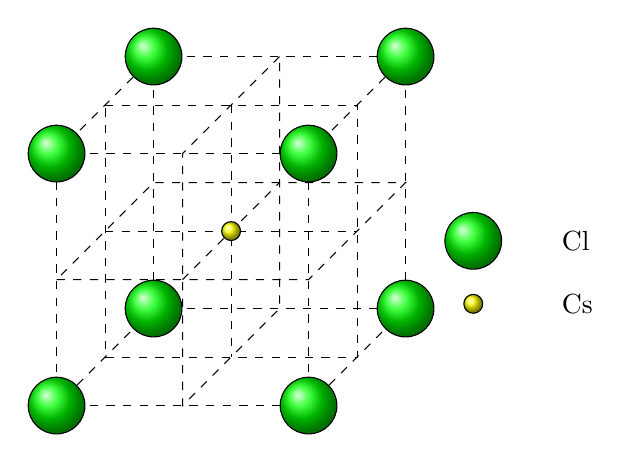
\begin{tikzpicture}[scale = 0.8]
%points on cube
\coordinate (A) at (0,0,0);
\coordinate (B) at (0,0,4);
\coordinate (D) at (0,4,0);
\coordinate (C) at (0,4,4);
\coordinate (E) at (4,0,0);
\coordinate (F) at (4,0,4);
\coordinate (H) at (4,4,0);
\coordinate (G) at (4,4,4);
%center of faces
\coordinate (I) at (0,2,2); %center of face ABCD
\coordinate (J) at (4,2,2); %center of face EFGH
\coordinate (K) at (2,4,2); %center of face DCGH
\coordinate (L) at (2,0,2); %center of face ABFE
\coordinate (M) at (2,2,4); %center of face CBGF
\coordinate (N) at (2,2,0); %center of face DAEH
%connectors
\coordinate (O) at (1,1,3);
\coordinate (P) at (1,3,1);
\coordinate (Q) at (3,1,1);
\coordinate (R) at (3,3,3);
%draw cube
\draw [dashed] (A) -- (B);
\draw [dashed] (B) -- (C);
\draw [dashed] (C) -- (D);
\draw [dashed] (D) -- (A);
\draw [dashed] (E) -- (F);
\draw [dashed] (F) -- (G);
\draw [dashed] (G) -- (H);
\draw [dashed] (H) -- (E);
\draw [dashed] (A) -- (E);
\draw [dashed] (B) -- (F);
\draw [dashed] (C) -- (G);
\draw [dashed] (D) -- (H);
%\draw [dashed] (2,2,2) -- (A);\draw [dashed] (2,2,2) -- (B);\draw [dashed] (2,2,2) -- (C);\draw [dashed] (2,2,2) -- (D);\draw [dashed] (2,2,2) -- (E);\draw [dashed] (2,2,2) -- (F);\draw [dashed] (2,2,2) -- (G);
\draw [dashed] (0,4,2) -- (4,4,2) -- (4,0,2)-- (0,0,2) -- cycle;
\draw [dashed] (2,4,0) -- (2,4,4) -- (2,0,4)-- (2,0,0) -- cycle;
\draw [dashed] (0,2,4)  -- (4,2,4) -- (4,2,0)  -- (0,2,0) -- cycle;
\draw [dashed] (I)  -- (J) ;
\draw [dashed] (K)  -- (L) ;
\draw [dashed] (M)  -- (N) ;
%Holes 
\coordinate (A1) at (0,4,2);
\coordinate (A2) at (4,4,2);
\coordinate (A3) at (4,0,2);
\coordinate (A4) at (0,0,2);
\coordinate (A5) at (2,4,0);
\coordinate (A6) at  (2,4,4);
\coordinate (A7) at (2,0,4);
\coordinate (A8) at (2,0,0);
\coordinate (A9) at (0,2,4);
\coordinate (A10) at (4,2,4);
\coordinate (A11) at (4,2,0);
\coordinate (A12) at (0,2,0);
\coordinate (A13) at (2,2,2);
 \def\COLORA{green};
  \def\COLORB{yellow};
%place non-atom cube corners
\shadedraw [ball color= \COLORA] (A) circle (0.45cm);
\shadedraw [ball color= \COLORA] (C) circle (0.45cm);
\shadedraw [ball color= \COLORA] (F) circle (0.45cm);
\shadedraw [ball color= \COLORA] (G) circle (0.45cm);
\shadedraw [ball color= \COLORA] (B) circle (0.45cm);
\shadedraw [ball color=\COLORA] (D) circle (0.45cm);
\shadedraw [ball color= \COLORA] (E) circle (0.45cm);
\shadedraw [ball color= \COLORA] (H) circle (0.45cm);



\shadedraw [ball color= \COLORB] (A13) circle (0.15cm);


\shadedraw [ball color= \COLORB, yshift=-2cm] (7,4,5) circle (0.15cm) node [right, xshift=1cm] {Cs};
\shadedraw [ball color= \COLORA, yshift=-2cm] (7,5,5) circle (0.45cm) node [right, xshift=1cm] {Cl};

%draw the center of each face
\end{tikzpicture}\end{center}

\end{question}
\begin{solution}
 \ce{Cs1Cl1}
 \hspace{0.1cm}\end{solution}\stepcounter{numA}
%%%%%%%%%%%%%%




%%%%%%%PROBLEM
\begin{question}[ID=\the\value{numA}]\SetQuestionProperties{section-title=\nameref{sec:units}}
Calculate the formula for the following unit cell:
\CaF  %\XeF   \CaTiO	\ZnS
\end{question}
\begin{solution}
 \ce{Cs1Cl1}
 \hspace{0.1cm}\end{solution}\stepcounter{numA}
%%%%%%%%%%%%%%


%%%%%%%PROBLEM
\begin{question}[ID=\the\value{numA}]\SetQuestionProperties{section-title=\nameref{sec:units}}
Calculate the formula for the following unit cell:
\XeF %  \CaTiO	\ZnS
\end{question}
\begin{solution}
 \ce{Cs1Cl1}
 \hspace{0.1cm}\end{solution}\stepcounter{numA}
%%%%%%%%%%%%%%


%%%%%%%PROBLEM
\begin{question}[ID=\the\value{numA}]\SetQuestionProperties{section-title=\nameref{sec:units}}
Calculate the formula for the following unit cell:
   \CaTiO	
\end{question}
\begin{solution}
 \ce{Cs1Cl1}
 \hspace{0.1cm}\end{solution}\stepcounter{numA}
%%%%%%%%%%%%%%
%%%%%%%PROBLEM
\begin{question}[ID=\the\value{numA}]\SetQuestionProperties{section-title=\nameref{sec:units}}
Calculate the formula for the following unit cell:
   \ZnS	
\end{question}
\begin{solution}
 \ce{Cs1Cl1}
 \hspace{0.1cm}\end{solution}\stepcounter{numA}
%%%%%%%%%%%%%%



{\raggedright\textsc{\textbf{Liquid state }}\par}
%
 %%%%%%%PROBLEM
\begin{question}[ID=\the\value{numA}]\SetQuestionProperties{section-title=\nameref{sec:units}}
Answer the following questions based on the image below:
\begin{inparaenum}[(a)]
\item Identify each meniscus as concave or convex %a: concave; b: convex
\item Which liquid has higher surface tension %b
\item Which liquid is more wettable (wets more) %a
\end{inparaenum}
\begin{center}\resizebox{.1\textwidth}{!}{\begin{tikzpicture}[pics/burette/.style={code={
     \tikzset{burette/.cd,#1}
     \def\pv##1{\pgfkeysvalueof{/tikz/burette/##1}}
     \pgfmathtruncatemacro{\imin}{\pv{min}+1}
     \pgfmathtruncatemacro{\imax}{\pv{max}}
     \draw[fill=blue!60,overlay] 
     (-\pv{width}/20,\pv{min}/10-\pv{min}/20-\pv{max}/20) -- 
     (-\pv{width}/20,\pv{fill}/10-\pv{min}/20-\pv{max}/20)
        to[/tikz/burette/top] coordinate[midway] (aux)
      (\pv{width}/20,\pv{fill}/10-\pv{min}/20-\pv{max}/20) -- 
      (\pv{width}/20,\pv{min}/10-\pv{min}/20-\pv{max}/20);
     \path[local bounding box=fill] 
      (aux)  (0,\pv{min}/10-\pv{min}/20-\pv{max}/20) 
     (0,\pv{fill}/10-\pv{min}/20-\pv{max}/20);
     \draw[densely dashed,thin]  
     (-\pv{width}/20,0|-fill.north) -- (\pv{width}/20,0|-fill.north);
     \draw foreach \XX [evaluate=\itest using {int(int(\XX/5)==int(\XX)/5?1:0)},
        evaluate=\jtest using {int(int(\XX/10)==int(\XX)/10?1:0)}] in {\imin,...,\imax}
      {(-\pv{width}/20,\XX/10-\pv{min}/20-\pv{max}/20) -- ++ (0.1+0.1*\itest,0)
        \ifnum\jtest=1 node[right]{$\XX$}\fi};
     \draw (-\pv{width}/20,\pv{max}/10+0.2-\pv{min}/20-\pv{max}/20) 
        -- (-\pv{width}/20,\pv{min}/10-\pv{min}/20-\pv{max}/20)
      (\pv{width}/20,\pv{max}/10+0.2-\pv{min}/20-\pv{max}/20) 
        -- (\pv{width}/20,\pv{min}/10-\pv{min}/20-\pv{max}/20);   
    }},burette/.cd,min/.initial=0,max/.initial=30,width/.initial=10,
    fill/.initial=10,top/.style={}]
 \path pic[yscale=2,semithick]{burette={min=7,max=21,fill=17,top/.style={bend right=20}}}
 (1.5,0) pic[yscale=2,semithick]{burette={min=7,max=21,fill=17,top/.style={bend left=20}}};
 \node[shift={(0em,-5em)}] (0em,0em) {A};
  \node[shift={(4em,-5em)}] (0em,0em) {B};

\end{tikzpicture}}\end{center}

\end{question}
\begin{solution}
\begin{inparaenum}[(a)]
\item  a: concave; b: convex
\item  b
\item  a
\end{inparaenum} \hspace{0.1cm}\end{solution}\stepcounter{numA}
%%%%%%%%%%%%%%
 %%%%%%%PROBLEM
\begin{question}[ID=\the\value{numA}]\SetQuestionProperties{section-title=\nameref{sec:units}}
Which of the following molecules present higher viscosity?
 \begin{center}\chemname{\chemfig{CH_3-C(-[2]CH_3)(-[6]Cl)-CH_3}}{A}\hspace{0.5cm}
 \chemname{\chemfig{CH_3-C(-[2]CH_3)(-[6]OH)-CH_3}}{B} \end{center}
\end{question}
\begin{solution}
B
 \hspace{0.1cm}\end{solution}\stepcounter{numA}
%%%%%%%%%%%%%%

 %%%%%%%PROBLEM
\begin{question}[ID=\the\value{numA}]\SetQuestionProperties{section-title=\nameref{sec:units}}
A liquid has a  enthalpy of vaporization of 30 $kJ/mol$ and a boiling point of 122$^{\circ}$C at 1.00 atm. Calculate its vapor pressure at 200$^{\circ}$C.
\end{question}
\begin{solution}
4.51atm
 \hspace{0.1cm}\end{solution}\stepcounter{numA}
%%%%%%%%%%%%%%







 %%%%%%%PROBLEM
\begin{question}[ID=\the\value{numA}]\SetQuestionProperties{section-title=\nameref{sec:units}}
What is the  enthalpy of vaporization of a liquid that has a vapor pressure of 500 torr at 100$^{\circ}$C and a boiling point of 90$^{\circ}$C at 460 torr?
\end{question}
\begin{solution}
9.3 kJ/mol
 \hspace{0.1cm}\end{solution}\stepcounter{numA}
%%%%%%%%%%%%%%


 %%%%%%%PROBLEM
\begin{question}[ID=\the\value{numA}]\SetQuestionProperties{section-title=\nameref{sec:units}}
The vapor pressure of a chemical at 32$^{\circ}$C is 0.86atm. Given that its heat of vaporization is 26kJ/mol, calculate the vapor pressure at 50$^{\circ}$C.
\end{question}
\begin{solution}
1.52atm
 \hspace{0.1cm}\end{solution}\stepcounter{numA}
%%%%%%%%%%%%%%

 %%%%%%%PROBLEM
\begin{question}[ID=\the\value{numA}]\SetQuestionProperties{section-title=\nameref{sec:units}}
Calculate the heat of vaporization of a chemical that doubles its vapor pressure when the temperature increases from 10$^{\circ}$C to 40$^{\circ}$C.
\end{question}
\begin{solution}
170kJ/mol
 \hspace{0.1cm}\end{solution}\stepcounter{numA}
%%%%%%%%%%%%%%

 %%%%%%%PROBLEM
\begin{question}[ID=\the\value{numA}]\SetQuestionProperties{section-title=\nameref{sec:units}}
For a chemical with heat of vaporization of 200kJ/mol, at what temperature will the vapor pressure be three times the value at 25$^{\circ}$C?
\end{question}
\begin{solution}
303$^{\circ}$Cl
 \hspace{0.1cm}\end{solution}\stepcounter{numA}
%%%%%%%%%%%%%%

 %%%%%%%PROBLEM
\begin{question}[ID=\the\value{numA}]\SetQuestionProperties{section-title=\nameref{sec:units}}
Given that the vapor pressure at 33$^{\circ}$C is 63mmHg for a chemical with molar heat of vaporization of 44kJ/mol, calculate the normal boiling point of this chemical--this is the boiling point at 760mmHg.
\end{question}
\begin{solution}
357$^{\circ}$Cl
 \hspace{0.1cm}\end{solution}\stepcounter{numA}
%%%%%%%%%%%%%%

 %%%%%%%PROBLEM
\begin{question}[ID=\the\value{numA}]\SetQuestionProperties{section-title=\nameref{sec:units}}
Order the following compounds from high to low vapor pressure ($P^{vap}$): \ce{NH3} ($\Delta H_{vap}$=23kJ/mol), \ce{CH4} ($\Delta H_{vap}$=8kJ/mol), \ce{C4H10} ($\Delta H_{vap}$=15kJ/mol)
\end{question}
\begin{solution}
$P^{vap}(\ce{CH4})$ > $P^{vap}(\ce{C4H10})$ > $P^{vap}(\ce{NH3})$.  
 \hspace{0.1cm}\end{solution}\stepcounter{numA}
%%%%%%%%%%%%%%
 %%%%%%%PROBLEM
\begin{question}[ID=\the\value{numA}]\SetQuestionProperties{section-title=\nameref{sec:units}}
Order the following compounds from high to low vapor pressure: \ce{C6H6} ($\Delta H_{vap}$=31kJ/mol), \ce{C6H5OH} ($\Delta H_{vap}$=39kJ/mol), \ce{H2O} ($\Delta H_{vap}$=41kJ/mol)
\end{question}
\begin{solution}
$P^{vap}(\ce{C6H6})$ > $P^{vap}(\ce{C6H5OH})$ > $P^{vap}(\ce{H2O})$.  
 \hspace{0.1cm}\end{solution}\stepcounter{numA}
%%%%%%%%%%%%%%









\end{multicols*}
\newpage
\begin{answersenvironment}
\begin{minipage}[c]{1\textwidth}
\begin{localsize}{10}
{\Large \bf Answers}
\SetupExSheets{
  headings = inline-nr , % numbered and inline
  counter-format = qu) , % numbers 1) 2) ... 
}
%\printsolutions 
\printsolutions[byID={1,3,5,7,9,11,13,15,17, 19,21,23,25,27, 29}]
\end{localsize}
\end{minipage}\end{answersenvironment}

\end{document}







